\documentclass[letterpaper,twocolumn,10pt]{article}
\usepackage{usenix2019_v3}

% For submission make this a noop

% to be able to draw some self-contained figs
\usepackage{tikz}
%\usepackage{parskip}
\usepackage{mathptmx}\renewcommand{\ttdefault}{cmtt}
\usepackage{amsmath}
\usepackage{wasysym}
%\setlength{\parskip}{1pt} % 1ex plus 0.5ex minus 0.2ex}
%\setlength\parskip{1pt}
\usepackage{graphicx} % http://ctan.org/pkg/graphicx
\usepackage{booktabs} % http://ctan.org/pkg/booktabs
\usepackage{xparse}   % http://ctan.org/pkg/xparse%don't print date
\NewDocumentCommand{\rot}{O{45} O{1em} m}{\makebox[#2][l]{\rotatebox{#1}{#3}}}%

\newcommand{\FigOverview}{
\begin{figure}[t]
    \centering
    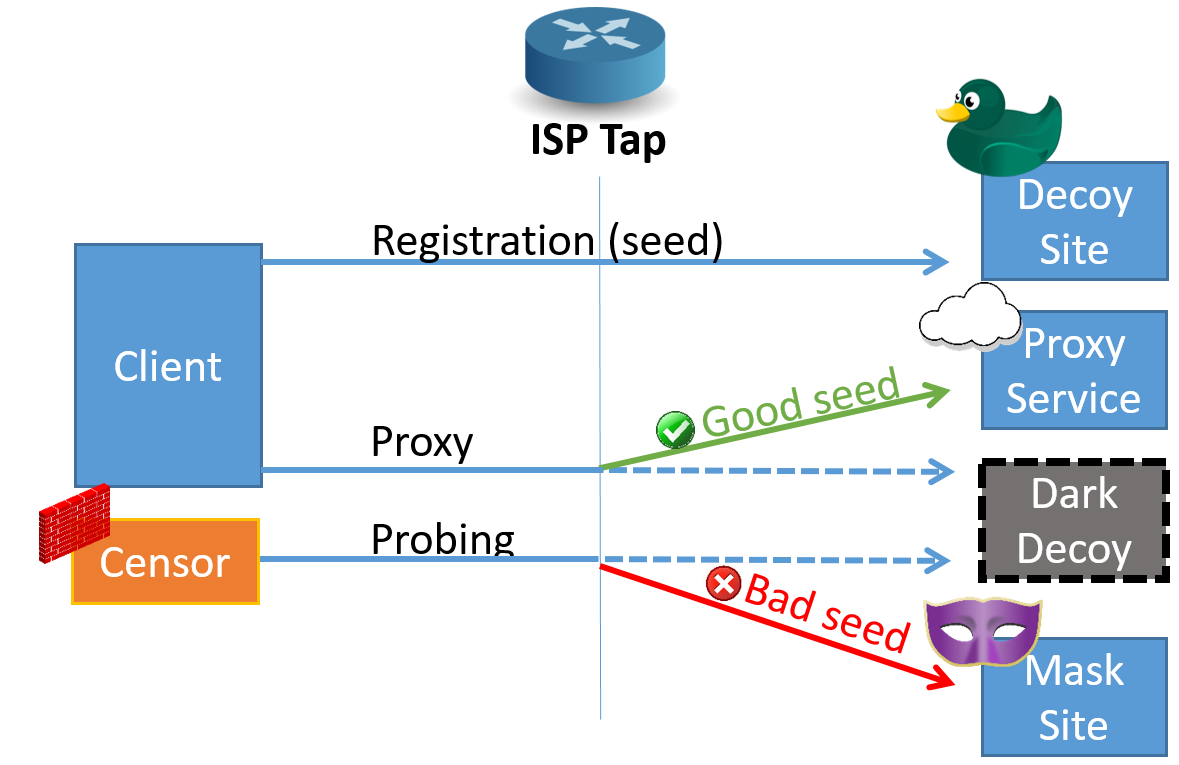
\includegraphics[width=\linewidth,clip]{figures/dark-decoy-overview.png}
    \caption{\textbf{\scheme Operations}\,---\,%
      \TODO{Caption}
    }
    \label{fig:overview}
\end{figure}
}

\newcommand{\FigHighLevel}{
\begin{figure}[t]
    \centering
    \vspace{-0.54in}
    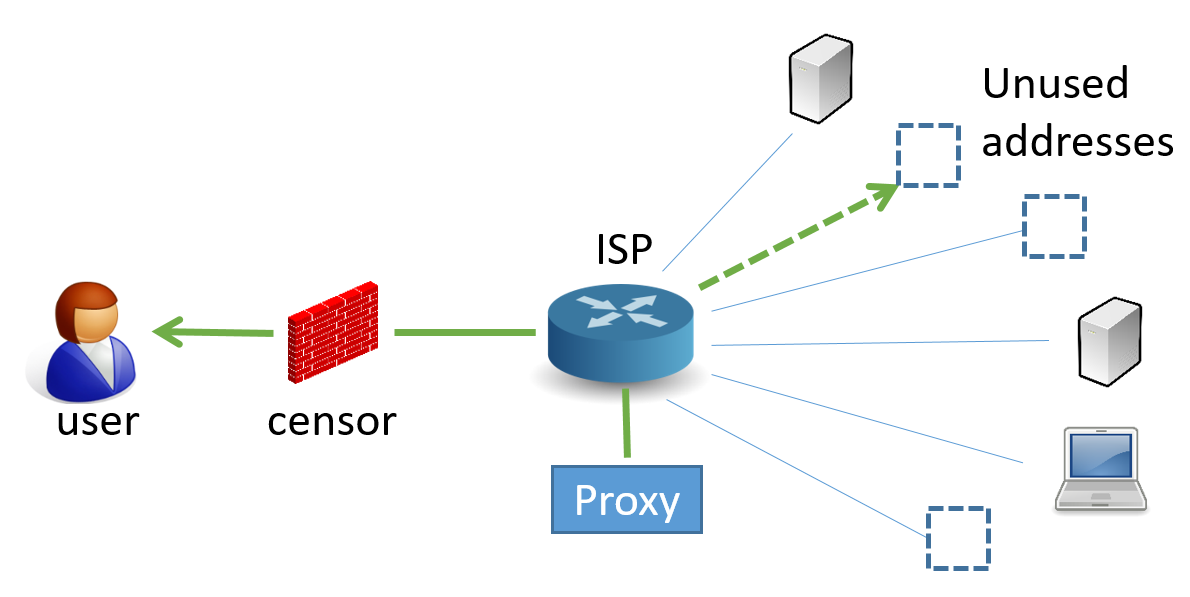
\includegraphics[width=\linewidth,clip]{figures/high-level.png}
    \caption{\textbf{\scheme Overview}---%
      An ISP deploys a \scheme station, which sees a passive tap of passing traffic.
      Following a steganographic registration process, a client can connect
      to an unused IP address in the ISP's AS, and the station will
      inject packets to communicate with the client as if there were a proxy server at that address.
    }
    \label{fig:highlevel}
\end{figure}
}

\newcommand{\FigUpload}{
\begin{figure}[t]
    \centering
    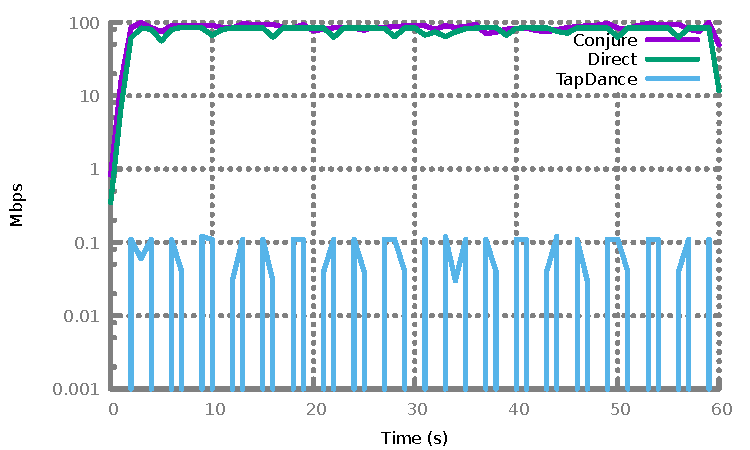
\includegraphics[width=0.90\linewidth,clip]{figures/bandwidth-up.pdf}
    \caption{\textbf{Upload Performance}\,---\, %
        We used iperf to measure the upload bandwidth for a direct connection, TapDance, and \scheme.
        As expected, TapDance's upload performance is several orders of magnitude lower than
        the link capacity, due to the overhead of frequent reconnects to the decoy.
    }
    \label{fig:upload}
\end{figure}
}

\newcommand{\FigDownload}{
\begin{figure}[t]
    \centering
    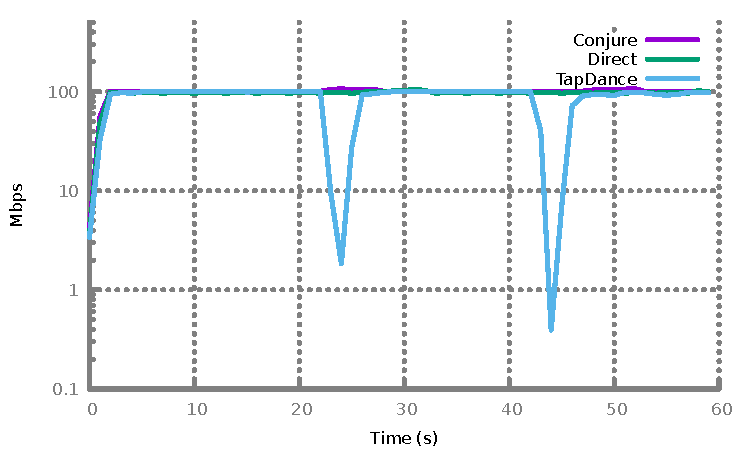
\includegraphics[width=0.90\linewidth,clip]{figures/bandwidth-down.pdf}
    \caption{\textbf{Download Performance}\,---\, %
        Using iperf, we compare the download performance of a direct connection, TapDance, and \scheme.
        While TapDance can achieve link capacity download, it still has to occasionally reconnect
        to the decoy, as seen by the periodic dips. These reconnects are more common the more data
        the client sends (e.g. requests or any upload data).
    }
    \label{fig:download}
\end{figure}
}


\newcommand{\FigTapBandwidth}{
\begin{figure*}[t]
    \centering
    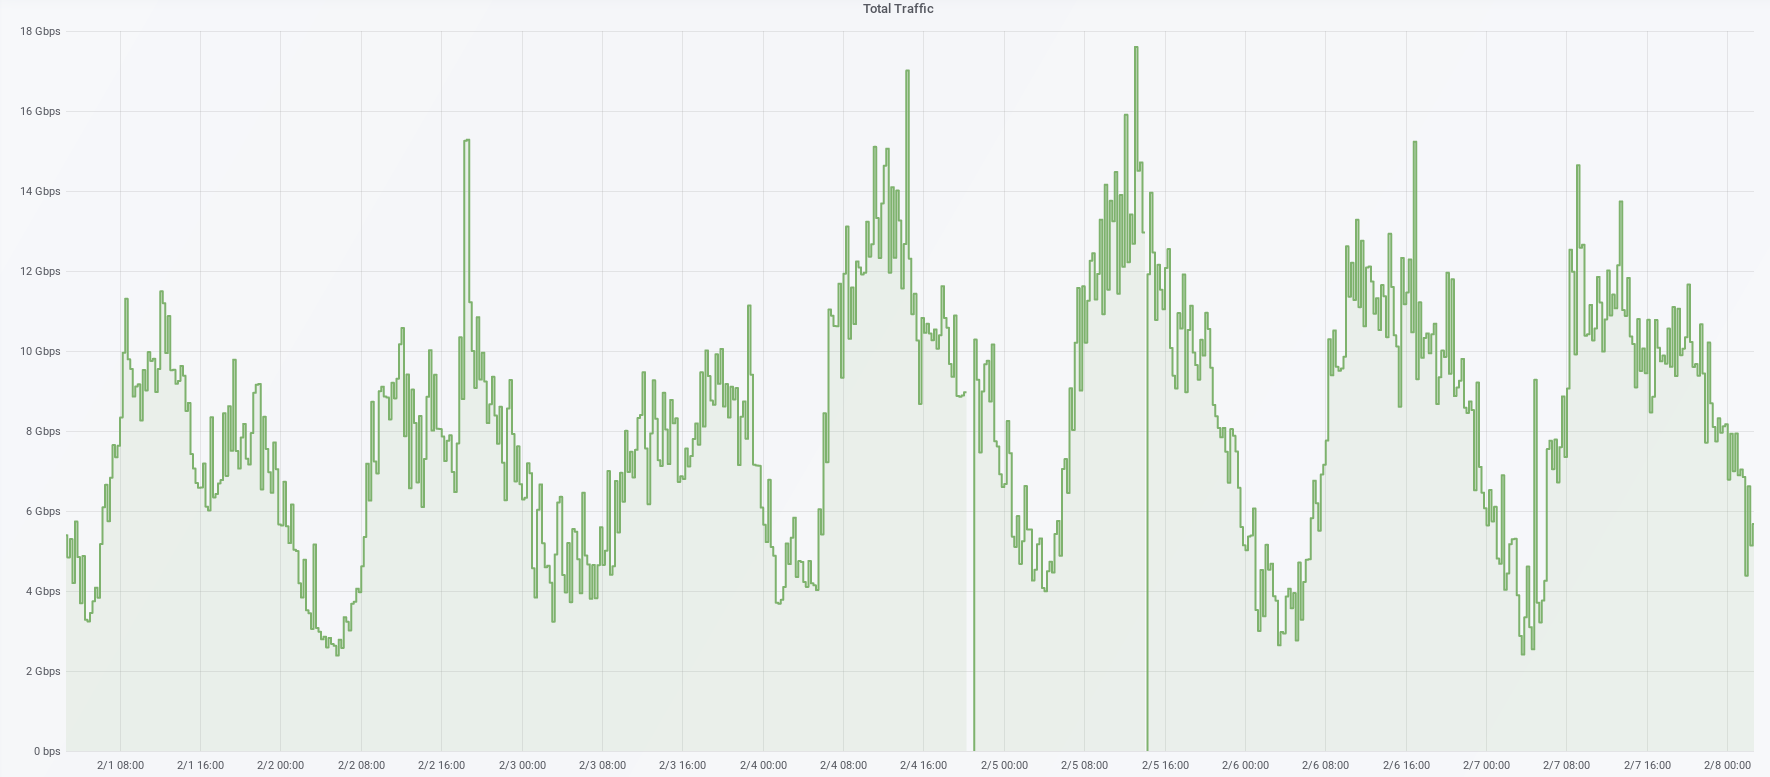
\includegraphics[width=0.90\linewidth,clip]{figures/decoy-tap-bandwidth.png}
    \caption{\textbf{Tap Bandwidth}\,---\, %
        We deployed our \scheme implementation in a realistic ISP testbed on a
        (full duplex) tap of a 10~Gbps router. As shown in a typical week, traffic
        ranges from 2-17~Gbps.
    }
    \label{fig:tap-bandwidth}
\end{figure*}
}




\newcommand{\FigIpBits}{
\begin{figure}[t]
    \centering
    \vspace{-0.5in}
    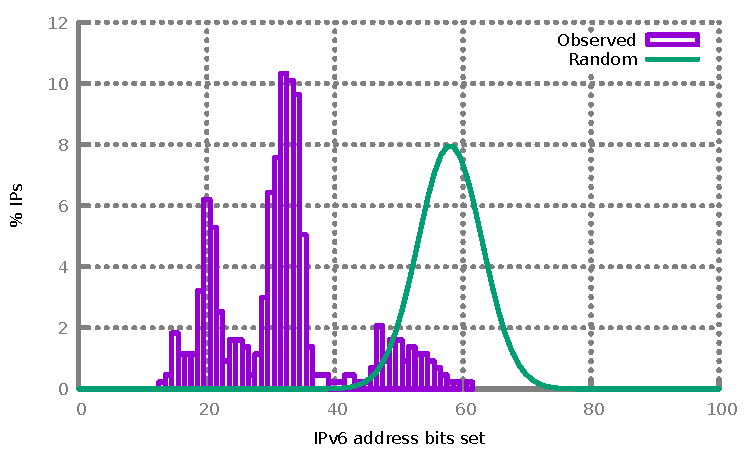
\includegraphics[width=\linewidth,clip]{figures/ip-bits-set-pdf.pdf}
    \caption{\textbf{IPv6 Entropy}---%
        We observed 30 minutes of IPv6 traffic on our tap to the /32 of the ISP's network.
        In each address observed, we counted the number of bits set, and compared this to
        randomly generated addresses. If the 96 non-network bits
        of each address were chosen randomly, we would expect to see a Binomial distribution
        (shown as Random). In practice, the distribution of observed IP addresses has much fewer
        bits set, suggesting that censors might be able to distinguish between dark decoy addresses
        and legitimate ones.
        %We note there are several /64 subnets that had many
        %addresses that appeared random (visibly overlapping the random distribution).
    }
    \label{fig:ipbits}
\end{figure}
}





\newcommand{\yes}{\CIRCLE}
\newcommand{\no}{\Circle}
\newcommand{\maybe}{\LEFTcircle}

\newcommand{\TabCompare}{
\begin{table*}[t]
    \centering
    \begin{tabular}{l|cccccccc}
            % Multiflow? Waterfall?
            & \rot{Telex~\cite{telex11}} &
            \rot{Cirripede~\cite{cirripede11}} &
            \rot{Decoy Routing~\cite{curveball11}} &
            \rot{TapDance~\cite{tapdance14}} & \rot{Rebound~\cite{rebound15}} & \rot{Slitheen~\cite{slitheen16}} & \rot{Waterfall~\cite{waterfall17}} & \rot{\textbf{\scheme}} \\
            \hline
                                      %Telex Cirr  DR     TD      RB    Slth   Water  DD
            No inline blocking        & \no & \no  & \no & \yes  & \no  & \no  & \no  & \yes \\
            Handles asym. routing     & \no & \yes & \no  & \yes & \yes & \no  & \yes & \yes \\
            Currently deployed        & \no & \no  & \no  & \yes & \no  & \no  & \no  & \no \\
            Replay attack resistant   &\yes & \yes & \yes & \no  & \yes & \yes & \yes & \yes \\
            Traffic analysis resitant &\no  & \no  & \no  & \no  &\maybe& \yes &\maybe& \no \\
            Uses unused addresses     & \no & \no  & \no  & \no  & \no  & \no  & \no  & \yes \\
    \end{tabular}
    \caption{\textbf{Comparing Refraction Networking schemes}\,---\,}
    \label{tab:compare}
\end{table*}
}



\newcommand{\FigImplementation}{
\begin{figure}[t]
    \centering
    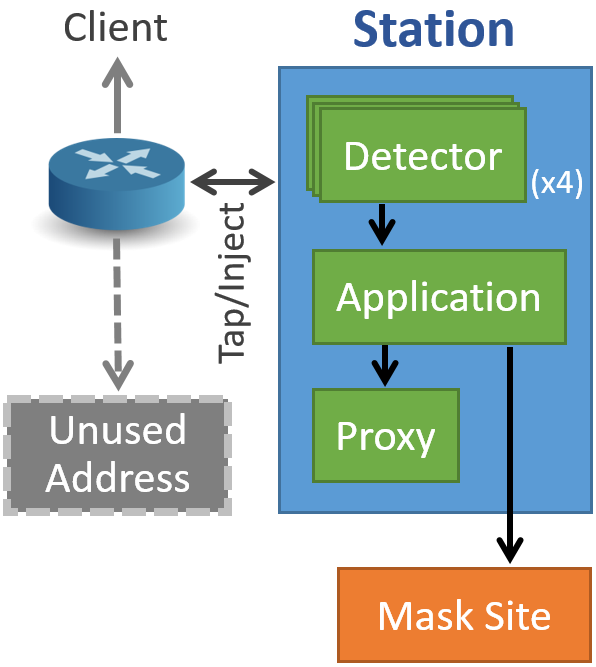
\includegraphics[width=0.7\linewidth,clip]{figures/implementation.png}
    \caption{\textbf{Station Architecture}\,---\,%
      \TODO{Caption}
    }
    \label{fig:implementation}
\end{figure}
}

\newcommand{\FigEvolution}{
\begin{figure}
  \centering
  \begin{subfigure}{\columnwidth}
    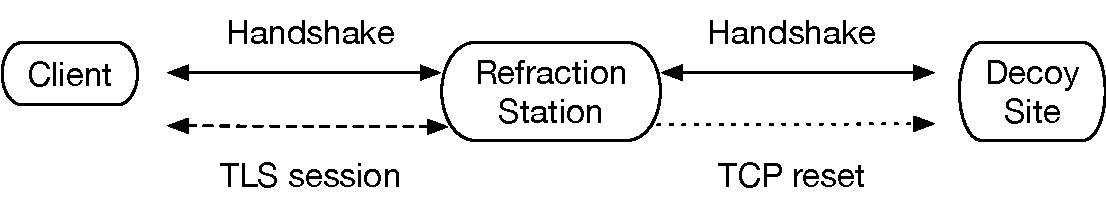
\includegraphics[width=\columnwidth]{figures/refraction-v1}
    \vspace{-3pt}

    \caption{\textbf{First generation systems} for Refraction Networking, such as Telex and Cirripede, operated as inline network elements, with the ability to observe traffic and block specific flows. ISPs worried that if the inline element failed, it could bring down the network.\looseness=-1}
    \label{fig:refraction-v1}
  \end{subfigure}
  \vspace{16pt}

  \begin{subfigure}{\columnwidth}
    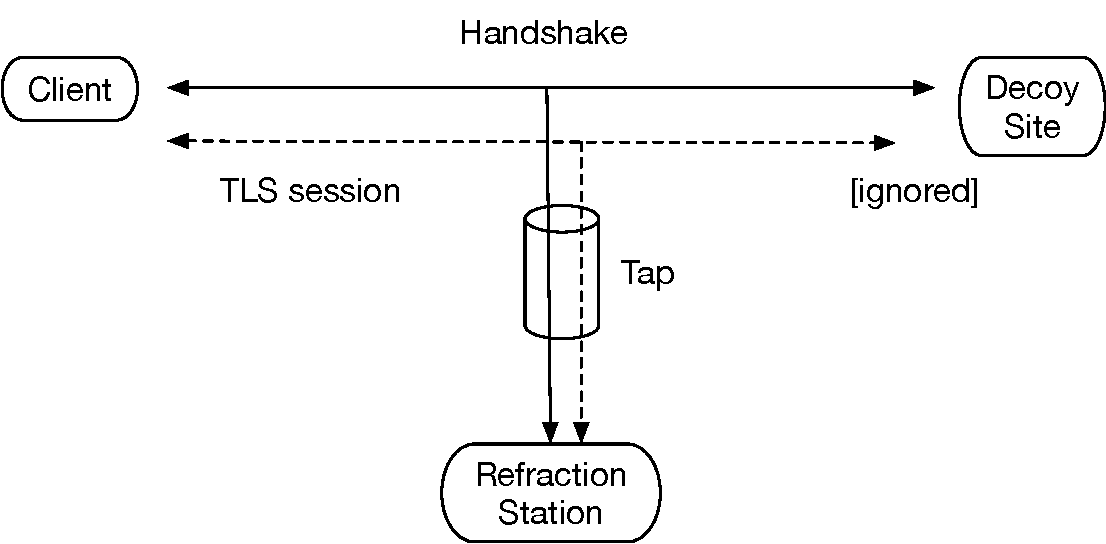
\includegraphics[width=\columnwidth]{figures/tapdance}
    \vspace{-3pt}

    \caption{\textbf{TapDance} is a second-generation Refraction Network scheme that operates without flow blocking, needing only to passively observe traffic and inject packets. TapDance has recently been deployed at a mid-size ISP, but the techniques used to silence the decoy site and participate in the client--decoy TCP connection mid-stream add significant complexity, performance bottlenecks, and detection risk.}
    \label{fig:tapdance}
  \end{subfigure}
  \vspace{16pt}

  \begin{subfigure}{\columnwidth}
    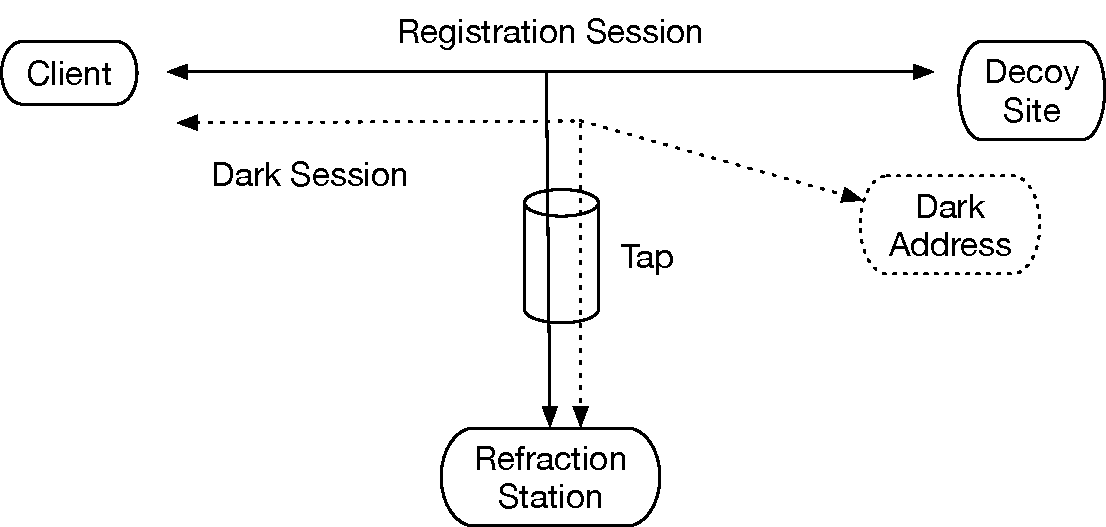
\includegraphics[width=\columnwidth]{figures/dark-decoys}
    \vspace{-3pt}

    \caption{\textbf{\scheme}, our third-generation Refraction Networking design, overcomes these limitations.  It uses two sessions. First, the client connects to a decoy site and embeds a steganographic registration message, which the station receives using only a passive tap.  Second, the client connects to a ``dark address'' where there is no running server, and the station proxies the connection in its entirety.}
    \label{fig:dark-decoys}
  \end{subfigure}

  \vspace{12pt}
  \caption{\textbf{Evolution of Refraction Networking Approaches}}
\end{figure}
}

\usepackage{subcaption}
\usepackage{cleveref}
\usepackage{microtype}
\SetExtraKerning{encoding=*,font=*}{\textemdash={120,120}} % Add space around emdashes
\usepackage[font=small]{caption}
\microtypecontext{spacing=nonfrench}
\usepackage{subcaption}
\usepackage{paralist}
\usepackage{xspace}
\usepackage{soul}
\newcommand{\note}[2]{\hl{[\textbf{#1:} #2]}\xspace}
\newcommand{\nikita}[1]{\note{nikita}{#1}}
\newcommand{\TODO}[1]{\hl{TODO: #1}\xspace}
\newcommand{\TK}{\hl{TK}\xspace}

% Slight JAH fix to stop URLs from breaking after ``http:''
\def\UrlBreaks{\do-\do\.\do\@\do\\\do\!\do\_\do\|\do\;\do\>\do\]%
 \do\)\do\,\do\?\do\'\do+\do\=\do\#}
\def\UrlBigBreaks{\do\:\do\/}%
\urlstyle{rm}

\renewcommand{\paragraph}[1]{\smallskip\noindent\textbf{#1\quad}}

\begin{document}

\date{}

% make title bold and 14 pt font (Latex default is non-bold, 16 pt)
%\title{\Large \bf Dark Decoys:
%  Conjuring Proxies from Unused Address Space}
\title{\Large \bf Conjure: Summoning Proxies from Unused Address Space}

%for single author (just remove % characters)
%\author{
%{\rm Your N.\ Here}\\
%Your Institution
%\and
%{\rm Second Name}\\
%Second Institution
%% copy the following lines to add more authors
%% \and
%% {\rm Name}\\
%%Name Institution
%} % end author

\maketitle

%\newcommand{\scheme}{Dark Decoys\xspace}
\newcommand{\scheme}{Conjure\xspace}

%-------------------------------------------------------------------------------
\begin{abstract}
%-------------------------------------------------------------------------------
Refraction Networking (formerly known as ``Decoy Routing'') has
emerged as a promising next-generation approach for circumventing
Internet censorship. Rather than trying to hide individual
circumvention proxy servers from censors, proxy functionality is
implemented in the core of the network, at cooperating ISPs in
friendly countries.  Any connection that traverses these ISPs could be
a conduit for the free flow of information, so censors cannot easily
block access without also blocking many legitimate sites.  While one
Refraction scheme, TapDance, has recently been deployed at ISP-scale,
it suffers from several problems: a limited number of ``decoy'' sites
in realistic deployments, high technical complexity, and undesirable
tradeoffs between performance and observability by the censor. These
challenges may impede broader deployment and ultimately allow censors to
block such techniques.

We present \scheme, an improved Refraction Networking approach
that overcomes these limitations by leveraging unused address space at
deploying ISPs. Instead of using real websites as the decoy destinations
for proxy connections, our scheme creates seemingly legitimate hosts
on demand, at IP addresses where no web server exists.
These phantom hosts are difficult for a censor to distinguish from
real ones, but can be used by clients as proxies.  We define the
\scheme protocol, analyze its security, and evaluate a
prototype using an ISP testbed.
Our results suggest that \scheme can be harder to block
than TapDance, is simpler to maintain and deploy,
and offers substantially better network performance.

\end{abstract}


\FigHighLevel

%-------------------------------------------------------------------------------
\section{Introduction}
%-------------------------------------------------------------------------------
% 1.5-2 pages



%Censorship circumvention still important
%-More countries blocking
%-Existing countries blocking more
%Internet censorship continues to hamper social progress throughout the world.

Over half of Internet users globally
now live in countries that block political, social, or religious content
online~\cite{fotn2018}.
%Existing circumvention strategies on shaky ground
%-domain fronting going away
%-active probing of existing proxies
%-Cenosrs fingerprinting known protocols
Meanwhile, many popular tools and techniques for circumventing such censorship
have ceased to function, because censors have evolved new ways to block them~\cite{ensafi-tor,great-cannon}
or infrastructure they rely on has become unavailable.

For example, domain fronting~\cite{meek} was a popular circumvention
strategy used by Meek (in Tor), as well as by the Signal secure messaging app to
get around censorship in countries where it was
blocked~\cite{signal,signal-domain-fronting}.
But in May~2018, Google and Amazon made both technical and policy changes to
their cloud infrastructures that removed support for domain
fronting~\cite{aws-front}. While meek
continues to use other cloud providers that (for now) continue to allow domain
fronting, Signal abandoned the strategy altogether~\cite{signal-back-on-front}.
There is an urgent need for new, more robust approaches to circumvention.

%Combined with censors' constant improvements in discovery and blocking
%techniques~\cite{ensafi-tor,great-cannon}, ...

%Importance of Refraction Networking
%-what it is, how it solves many of the above problems
%-acknowledge challenge of ISP deployment, cite TapDance deployment as only refraction technology that has overcome this challenge so far
A family of techniques called Refraction Networking~\cite{telex11,cirripede11,curveball11,tapdance14,rebound15,slitheen16,waterfall17}, formerly known
as Decoy Routing, has made promising steps towards that goal.
These techniques operate in the network's core, at cooperating Internet Service Providers
(ISPs) outside censoring countries~\cite{refraction-site}.  Clients access circumvention service by connecting to a ``decoy site''---any uncensored website for which the connection travels over a participating ISP\@.  Upon recognizing a steganographic signal from the client, the ISP modifies the connection response to return censored content requested by the user.
Censors cannot easily block access without also blocking legitimate connections to the decoy sites---collateral damage that may be prohibitive for censors if Refraction is widely deployed~\cite{robinson2013collateral}.

However, deploying such schemes is more difficult than with most
edge-based circumvention techniques, since ISPs must be convinced to
operate the systems in their production networks.  To date, only
TapDance~\cite{tapdance14}, one of six Refraction Networking
proposals, has been deployed at ISP scale~\cite{frolov2017isp}.

TapDance was designed for ease of deployment.
Instead of in-line network devices required by earlier schemes, it
calls for only a passive tap.
This ``on-the-side'' approach, though much friendlier from an ISP's
perspective, leads to major challenges when interposing in an ongoing
client-to--decoy connection:
\begin{compactitem}
\item Implementation is complex and error-prone, requiring kernel
  patches or a custom TCP stack.
\item To avoid detection, the system must carefully mimic
  subtle features of each decoy's TCP and TLS behavior.
\item The architecture cannot resist active probing attacks, where the
  censor sends specially crafted packets to determine whether a
  suspected connection is using TapDance.
\item Interactions with the decoy's network stack limit the length and
  duration of each connection, forcing TapDance to multiplex
  long-lived proxy connections over many shorter decoy
  connections. This adds overhead and creates a traffic pattern
  that is challenging to conceal.
\end{compactitem}

%Challenges remain in Tapdance:
%-Censor can fingerprint decoy sites
%-Decoys themselves are limited (e.g. a few dozen in many cases)
%-Can't have long-lived connections (performance and observability issue)
%-Other performance limits (upload limit, TCP window size)

%% AH: I'm not sure I buy this limited decoys argument. If there are
%% few decoys, there is little collateral damage of blocking
%% everything in the AS, and \scheme is at a big disadvantage too.
%The use of real-world decoy sites also presents practical problems: If
%decoys are limited or not particularly important, it may be easy for a
%censor to block them altogether without much collateral damage.

%Dark decoys solve these issues
%-Create new decoys from ``dark'' (unused) address space
%-Clients register (via TapDance-like or other robust protocol (email, blockchain, whatever))
%-Connect to custom IP address, talk whatever protocol client/station agrees on

\smallskip

In this paper, we present \textbf{\scheme}, a Refraction
Networking protocol that overcomes these challenges while retaining
TapDance's ISP-friendly deployment requirements.
Our key innovation is an architecture that avoids
having to actively participate in client-to-decoy connections.

%\TODO{more precise:}
In our scheme (Figure~\ref{fig:highlevel}), clients
request the creation of phantom hosts in the ``dark''
or unused address space of the deploying ISP. Once registered, clients
can connect to these phantom hosts IP addresses as if they were real
proxy servers. The ISP station acts as the other end of these connections, and
responds as if it were a legitimate site or service. To the censor,
these phantom hosts appear as legitimate sites or services, and even
active probes will not reveal information that would allow the censor to
block them.

%% requests service
%% by embedding a steganographic registration message in a TLS handshake
%% with a decoy site. This message, which the ISP station can passively
%% observe using a private key, uniquely determines an IP address within
%% the ISP's address space. If there is no server running at that address,

%One-time use address advantages:
%-Censor cannot actively probe ahead of time (especially in IPv6), making it hard to fingerprint
%-Decoys are now virtually unlimited (or limited only by address space)
%-Connection can live as long as we want
%-No pesky TCP/TapDance-y limits

Phantom hosts are cheap to create, allowing for discardable or even one-time-use
proxy servers. This greatly increases the cost for censors to
block, as they must detect and block in real time. Meanwhile, even a censor that
can detect 90\% of phantom hosts does not significantly increase the cost to the
circumvention system, giving \scheme an advantage in the censor/circumventor
cat-and-mouse game.
\scheme supports both IPv4 and IPv6, though we note that the technique is especially
powerful in IPv6, where censors cannot exhaustively scan the address space
ahead of time to identify addresses that change behavior.
Because we fully control the transport connection, connections can live as
long as needed, without the complexity faced by TapDance.

%TODO:
%Requirements/Challenges
%-Censor can't be able to distinguish between dark decoy and legitimate hosts
%    (otherwise they block all dark decoys)
%    -Includes active probing: censor shouldn't be able to register existing IP
%-Disruption avoidence: Want to pickup even for used addresses
%    -Otherwise, censor probes to find truly unused address space and blocks
%    -But can't disrupt legitimate services
%    -Can overcome by limiting pickup to the registering client (but spoofing challenges...)
%    -Note: also likely solved by the client-sends-SNI in the Mask site application...

% We implement it, it works...

We introduce the \scheme protocol (Section~\ref{sec:architecture})
and analyze its security, finding that it resists a broader
range of detection attacks than TapDance.
We have implemented a prototype implementation (Section~\ref{sec:implementation})
and deployed it on a 10~Gbps testbed similar to the TapDance
deployment~\cite{frolov2017isp}.  Compared to TapDance, we find that
\scheme has reduced complexity and substantially improved performance
(Section~\ref{sec:evaluation}).  We believe that these advantages
make \scheme a strong choice for future Refraction Networking deployments.

\section{Background}

Refraction networking operates by injecting covert communication inside a
client's HTTPS connection with a reachable site, also known as a decoy site. In
a regular HTTPS session, a client establishes a TCP connection, performs a TLS
handshake with a destination site, sends an encrypted web request, and
receives an encrypted response. In refraction routing, at least one direction
of this exchange is observed by a \emph{refraction station}, deployed at
some Internet service provider (ISP). The station watches for a covert signal from
the client that this connection is to be used for censorship circumvention.
Upon seeing the signal, the station will take over the HTTPS session,
and establish a proxy session with the client that can then be used for covert
communication.

\FigEvolution

One of the key challenges for refraction networking is in taking over a session. The station must start responding to the client's traffic as if it were the decoy destination, and at the same time prevent the destination from sending its own responses back to the client. A simple approach is to have the refraction station act as an inline transparent proxy (Figure~\ref{fig:refraction-v1}) that forwards the traffic between the client and the decoy site. After a TLS handshake has been completed, the station terminates the connection with the decoy site by sending a TCP reset and takes over the session with the client.

An inline element, however, can significantly affect the reliability and performance of the regular, non-refraction traffic of an ISP. Cirripede~\cite{cirripede11} and Telex~\cite{telex11} attempted to mitigate this by dynamically adding router rules to forward only a subset of traffic from a registered client or an active session through the element, but this nevertheless presented a deployability challenge.

TapDance~\cite{tapdance14} offered an alternative design that did not require the blocking or redirection of traffic, but used a mirror port instead (Figure~\ref{fig:tapdance}). In TapDance a client sends an incomplete HTTP request, which causes the decoy site to pause waiting for more data while the station takes over the connection in its place. After a client would receive a packet initiated by the station, its TCP sequence numbers would become desynchronized with the decoy site, causing the decoy to ignore the packets sent by the client.

This approach reduced the barriers to deployment and TapDance was used in production during a pilot study, serving upwards of 50\,000 real-world users~\cite{frolov2017isp}. 
%\nikita{worth mentioning that it's being used in production again? we don't have a public ref for that though.} 
The tap-based approach, however, has some disadvantages. A decoy site will only ignore packets as long as the sequence numbers stay within its TCP window, and will terminate the connection after a timeout. Frolov et al.\ report that in their pilot, they eliminated roughly a third of potential decoy sites due to their measured window or timeout values being too small~\cite{frolov2017isp}. Even so, sessions that try to upload non-trivial data amounts (in excess of about 15\,KB) or last longer than the timeout value (ranging from 20--120\,s) require the user to create new refraction connections, adding overhead, complexity, and opportunities for errors. Additionally, keeping the connections to the decoy site open for tens of seconds uses up the site's resources; Frolov et al.\ found that a default configuration of the Apache web server would only keep 150 simultaneous connections open, while the pilot deployment would often result in dozens of connections to the same decoy site, creating a scaling concern.

\scheme is able to avoid these problems by creating proxies at unused IP addresses, allowing the station full control over a host it has created, rather than forcing it to mimic an already existing decoy (Figure~\ref{fig:dark-decoys}).
%The registration session is used to send a signal to the station to let RS know that the client plans to use dark sessions and to establish a seed to be used in future communications (\cref{XXX}); the RS only passively observes this connection without any interference. The dark session connects to a dark address that is not routed to any host; the RS instead acts as a remote endpoint for the entirety of the connection, starting with the TCP handshake. 
This design obviates the need for taking over a session already in progress, which both simplifies the implementation and eliminates certain attacks, as we will discuss in Section~\ref{sec:attacks}.

\paragraph{Registration Signal} In all implementations of refraction networking, a client must send a covert signal to the station to initiate communication. This covert signal is  embedded inside communication fields that must be indistinguishable from random by a censor without access to a secret/private key available to the station. Past implementations have used TCP initial sequence numbers~\cite{cirripede11}, the ClientRandom field inside a TLS handshake~\cite{curveball11,telex11}, and the encrypted body of an HTTPS request~\cite{tapdance14}. In principle \scheme can use any of these mechanisms for registration, but in our prototype we used the HTTPS request body as it offers the greatest flexibility for the amount of data that can be sent with the registration.



\section{Threat Model}
% 0.25 page


Our deployment model is identical to that of TapDance: we only require a passive
tap at the deploying ISP, and the ability to inject (spoofed) traffic from phantom
hosts.
Furthermore, we assume
asymmetric routing (i.e. that the tap can sometimes only see packets from but not to the
client).
However, we assume a stronger threat model for the adversary than
TapDance, as our design resists active attacks.


We assume the censor can block arbitrary IP addresses and networks, but faces a
cost in doing so if it blocks potentially useful resources. In particular, we
assume it is difficult for the censor to have complete knowledge of legitimate
addresses used, and so instead resorts to a blacklist approach to blocking
proxies and objectionable content.
Whitelists are expensive for censors to maintain and can stifle
innovation, and are rarely employed by censors.


We assume that the censor can know what network the \scheme station(s) are
deployed in and the prefixes phantom hosts are selected from, but that blocking those
networks outright brings a collateral
damage the censor is unwilling to suffer. Instead, the censor aims to identify
the addresses that are phantom hosts, and block only those.

We assume the censor can use the client to register and access its own phantom
hosts, but that these will not reveal the phantom hosts of other users. The
censor can also actively probe addresses that it sees users accessing, but can
not enumerate the entire ISP prefix (e.g. a /32 IPv6 prefix contains
$2^{96} addresses$).

Finally, we assume the censor can replay or preplay any connections that it
suspects involve phantom hosts (or their registration) in an attempt to confirm.
However, the censor wishes to avoid disrupting any connections before it
knows for certain they are from \scheme clients, lest they disrupt legitimate
connections. This means that injecting false data or corrupting TLS sessions is
outside the scope of the censor, but that the censor can send non-disruptive
probes (such as stale TCP acknowledgements or other packets that would normally
be ignored). We emphasize that TapDance is observable by censors that can send
TCP packets in suspected connections, but that our protocol is robust against
this class of censor.

%-Censor can block arbitrary addresses (or networks), but faces a cost in doing so (collateral damage)
%-Censor can know what network deploys the dark decoy station
%-Censor knows the dark decoy prefixes distributed in the client, but they contain legitimate hosts
%-Censor can use the client
%-Censor can active probe limited sets, but cannot enumerate the entire prefix (i.e. IPv6 /32)
%-Censor can active probe or (p)replay connections it suspects


\section{Architecture}
\label{sec:architecture}
% 3 pages

\scheme involves three main steps. First, clients \textbf{register} with the
ISP station,
and agree on the phantom host IP address that will be used. Next, the client
connects to the agreed upon address, which is terminated by an
\textbf{application} running on the station. Finally, the client \textbf{proves}
to the application that it was the same client that registered (and not a censor
attempting to probe), and is able to use the application as a proxy.

Similar to previous schemes, our design does not require expensive in-line
flow blocking, and can be accomplished with only a passive tap at the ISP.
Our architecture is also modular, in that the registration and application steps operate
independently, allowing a wide range of flexibility to evade censors. We
describe each of these components.

\subsection{Registration}

Clients can register intent to use the proxy in several covert ways. For
instance, they could use email or other existing intermittently available proxies
to register. In this section, we use a form of Refraction Networking similar to
TapDance to register directly with the station.

Registration is unidirectional (client to server) and does not require any
acknowledgement of receipt. To ensure receipt, clients can attempt to register
multiple times (possibly via multiple methods) with the same information, and expect
that one gets through.

\medskip

To register, clients connect to a \textbf{decoy} site that supports TLS. They
complete the handshake, and send a normal HTTPS request that embeds a special
steganographic \textbf{tag} in the ciphertext of the request. We use
the same technique used in TapDance's covert ciphertext channel\footnote{Section 3 in
TapDance~\cite{tapdance14}} to embed the tag, but we purposefully have the client
send a complete request (rather than incomplete), allowing the decoy server to respond.
The steganographic tag is only visible to the ISP station, which can see the tag using its
private key. Unlike in TapDance, the \scheme station can passively observe
the tag, and does not need to respond to it (which requires mimicking the
decoy)


The tag contains a public key (encoded to be indistinguishable from random using
Elligator~\cite{elligator}), and a message encrypted under the shared secret
derived from a key exchange with the station's long-term public key hard-coded
in the client software. The station uses its private key to compute the same
shared secret from the (decoded) public key, and decrypts the message in the
tag. The censor, without knowledge of either the station or client's private
key, cannot derive the shared secret, preventing it from being able to decrypt
the message, or even learn of its existence.


Inside the message, the client communicates a random \textbf{seed}, and other
configuration-specific information, such as flags to signify version, feature
support, and a set of IPv6 network prefixes that the client knows can be used
for phantom hosts (previously distributed publicly).
The client and server hash the seed to determine which specific
IPv6 address from the set of prefixes will be used and registered as a phantom host. It may seem intuitive to instead have the client
send the specific IP address to register, but allowing the client arbitrary
choice also allows the censor to register suspected phantom hosts and block them if
they pick up. 
By using a hash of a seed, the censor would have to pre-image the hash to
obtain a seed it could use to register for a desired IP address.
It also gives a
secret (the seed) that only the client and station know, even after the client
connects to the phantom host address.

Once the phantom host IP address has been selected, the station watches for
packets destined to that address, and forwards them onto the phantom host
\textbf{application}. The station can also optionally ignore packets not from
the source IP address of the registering client, so that to a probing censor
from a different IP address,
the phantom host appears to be firewalled off from all but the client. We note
this is not a robust solution: censors have previously been observed taking over
IP addresses of clients~\cite{ensafi-tor}. We instead address active probing in
the application.

\subsubsection{IPv6 vs.\ IPv4 Phantom Hosts}


Phantom host IP addresses must be derived from network blocks that are routed (so they pass
the ISP station) and contain other legitimate hosts (so that censors cannot
block the entire network without collateral damage).
Because of the large number of IPv6 addresses, even
relatively small network prefixes have astronomical numbers of addresses: a
single /32 prefix has $2^{96}$ possible addresses. Therefore, client-chosen
seeds have negligible probability of corresponding to addresses that are already
being used by legitimate hosts. This allows us to select phantom host addresses
from network prefixes that contain
legitimate hosts---crucial to discouraging the censor from blocking them
outright---without worry that registrations could interfere with legitimate
services.

In addition, the use of IPv6 prevents censors from exhaustively probing
potential phantom host network prefixes ahead of time to learn the full set of
legitimate sites in the network.

\paragraph{IPv4}
While \scheme composes well with IPv6, we can also support IPv4,
at the cost of being vulnerable to active probing by the censor.
We emphasize that TapDance is already
vulnerable to active probing attacks~\cite{tapdance14} that \scheme defends
against when using IPv6. However, in IPv4, there are substantially fewer
addresses, allowing censors to easily enumerate network prefixes that pass by
the ISP station and measure legitimate sites. Furthermore, the small address
space makes it much easier to pre-image the hash used to derive IP addresses
from the seed. Registering a specific IPv4 address in an IPv4 /16 subnet will
take only an expected $2^{16}$ hashes for the censor to achieve. This would let
attackers register legitimate hosts as phantom hosts, potentially disrupting
legitimate service. If the station refused to pick up for addresses that
correspond to legitimate hosts (measured by scanning during registration), then
censors could use this as an oracle for distinguishing legitimate sites from
phantom hosts. Still, IPv4 \scheme offers many performance, flexibility, and
simplicity benefits over TapDance, though they are both vulnerable to active
probing attacks.


%While address utilization in IPv4 is quite high (all blocks have been allocated
%at the RIR level), the fraction of addresses that respond to TCP connections on
%a given port is quite low: even popular ports like 443 (use by TLS) have less
%than 2\% of IPv4 hosts respond to connection requests. This leaves a large
%number of hosts available to use as dark decoys. However, if a client registers
%a dark decoy address that is already happens to be used by an existing host,
%there will be multiple responses when the client tries to connect, and the
%connection will fail. However, this failure is still limited to the registering
%client, as the application only responds to the IP of the client that
%registered. In IPv6, the odds of picking a legitimate host are negligible: with
%a /32 prefix of IPv6, there are $2^{96}$ addresses to choose from.
%\nikita{/32 is pretty big, e.g. UIUC only has a /48}


\subsection{Applications}


Once the client has registered, packets sent to the phantom host IP address are
passed to the \textbf{application} running on the station. The application has
two main jobs: first, it must look like an innocuous legitimate service to the
censor, and second must allow the client to use it as a proxy.

Any protocol that satisfies these criteria can be used as an application. For
instance, \texttt{obfs4}~\cite{obfs4} is a pluggable transport used by
Tor~\cite{tor} that could be
modified to meet these needs: it requires each endpoint to have knowledge of a
shared secret (which we can derive from the seed shared by the client and
station during registration), and attempts to be a protocol with no discernible
fingerprint. Probing censors that do not have the shared secret receive no
response, while clients that have the secret can communicate with the proxy.

However, even though \texttt{obfs4} is indistinguishable from random, there are
still known attacks that can differentiate it from other
traffic~\cite{wang2015seeing}. While we have yet to see evidence of such attacks
employed in practice by censors, we consider two alternatives built on TLS.


\FigOverview

\subsubsection{Mask Sites}

TLS is a natural protocol for \scheme applications, because it is ubiquitous on
the Internet (making it difficult for censors to block), while also providing
strong cryptographic protection against passive and active network adversaries.
However, there are several challenges to make it robust against censors that
wish to block a particular service.

This is because TLS sends important server-identifying content in plaintext
during the TLS handshake. This includes the Server Name Indication (SNI) in the
Client Hello message that sends the domain name of the server, and the
X.509 Certificate sent by the server.

To evade censors, we must send a plausible SNI value (sending no SNI is
uncommon and easily blocked---study conducted using Colorado University network
infrastructure shows that only 1\% of all TLS connections coming in and out of 
campus do not carry the
SNI extension~\cite{tls-fingerprint}), and we must have the server respond with
a plausible (and corresponding) certificate. Even if we manage to avoid sending
either in the clear, censors could actively probe the server in a
way that would normally elicit a certificate.


We therefore attempt to mimic an existing \textbf{mask site}, by relaying
traffic between the client and a selected mask website. To a censor, this site
will be indistinguishable from the legitimate mask site, making it difficult for
them to block without potentially blocking the actual site. TLS connections to the
application will terminate exactly as connections to the mask site would, with the
application acting as a transparent proxy between the client and mask site.
However, this leaves the application unable to introspect on the contents of the
TLS connection to the mask site, as it does not have the client-site shared
secrets, and it cannot overtly man-in-the-middle the connection before knowing
it is communicating with the legitimate client (and not the censor).


To accomplish this, the client changes the shared secret it derives with the
mask site to something that the application can also derive. The client's first
\texttt{Application Data} packet is thus encrypted under a different secret than
the client/mask site secret. Specifically, the client uses the \textbf{seed}
sent during registration to derive the pre-master secret for the connection.
This is hashed along with the client and server randoms of the current (mask
site) TLS connection to obtain the master secret that determines
encryption/decryption/authentication keys.

The application can determine if the client did this by trial decryption with
the master secret derived from the known \textbf{seed}. If it succeeds, the
client has proved knowledge of the \textbf{seed}, and the application can
respond as a proxy. If not, the application simply continues to forward data
between the client and the mask site. As the censor does not have knowledge of
the \textbf{seed} used in registration, it cannot coerce the application to
appear as anything besides the mask site.


\subsubsection{Mask Site Selection}

Selecting which sites to masquerade as must be done carefully to avoid censors
being able to detect obvious choices. For example, if a small university network
has a phantom host in their network that appears to be \texttt{apple.com}, it
would be easy for a censor to block as a likely non-legitimate host. Likewise,
if a phantom host at an IP address pretends to be a domain (\texttt{example.com}) that
globally resolves to a single different IP address, the censor could also
identify and block the phantom host.

\paragraph{Nearby sites.}
One strategy for selecting mask sites to mimic is to pick websites that are
legitimately hosted in or near the network of the phantom host addresses. This
effectively creates copies of legitimate sites, with the censor unable to
determine which copies are real and which are the phantom hosts. However, as
mentioned, other signals such as DNS may reveal the true mask site.

\paragraph{Popular sites.}
An alternative strategy is to use popular sites, such as those from the Alexa
top site~\cite{alexa-top500} list. As mentioned previously, it may be wise to avoid
sites that are obviously not hosted in the phantom host address range, such as
large companies that run their own data centers and own their own ASN.
The list could also be filtered to domains that resolve to different IP
addresses from different vantage points, making it harder for a censor to know
if a phantom host corresponds to a domain's IP.

\paragraph{Passive observation.}
The ISP tap could also collect sites by passively observing DNS requests, TLS
SNI, or certificates that pass by. This would allow for building a realistic set
of sites that are plausibly in the vicinity of the phantom host addresses
that pass by the tap. It also has the added bonus of being able to discover
IPv6 addresses that could be used as decoys (for registration), where active
scanning would be infeasible.

In practice, clients can often try phantom hosts/mask sites over
several attempts, as blocking the client outright may negatively impact other
unrelated users behind the same network (e.g. in the case of NAT). Thus, even a
censor that can block most (but not all) mask site only delays access, and
doesn't prevent it outright.

\subsubsection{Encrypted SNI}
\label{esni}

TLS~1.3~\cite{tls13} offers several features that may greatly simplify 
\scheme application design. For instance, TLS~1.3 handshakes include encrypted
certificates, potentially obviating the need to impersonate mask sites.
Unfortunately, TLS~1.3 currently still sends the SNI in the (plaintext) Client
Hello, meaning we would still have to choose a realistic domain to fool a
censor.

However, there are proposals to encrypt the SNI in the Client Hello~\cite{esni},
though none have been implemented or deployed as of early 2019. Nonetheless,
if widely adopted, Encrypted SNI (ESNI) would offer a powerful solution for
\scheme applications by allowing the domain to remain hidden from the censor.
While the censor could still try to actively probe with guesses for the SNI,
servers could respond with generic ``Unknown SNI'' errors. If such responses
were common for incorrect SNI, the censor's efforts to identify phantom hosts
would be frustrated.

\subsubsection{WebRTC}
\label{sec:webrtc}

Phantom hosts could also pretend to be clients instead of servers. This may
potentially give censors less to block on, as actively probing clients is common
to return few or no open ports. Nonetheless, a censor may be hesitant to block
client-to-client communication, as it could block peer-to-peer applications as
well as many video conferencing protocols. WebRTC is a
natural choice for a client-to-client protocol in censorship circumvention,
and is used in existing censorship circumvention schemes like
Snowflake~\cite{snowflake}. \scheme could also use WebRTC as the
application protocol, convincing the censor that two clients are communicating.

\section{Implementation}
\label{sec:implementation}

We implemented the \scheme protocol and tested it in a 10~Gbps ISP testbed
with real traffic. Similar to TapDance~\cite{tapdance14}, we used PF\_RING to
consume the 10~Gbps link, and feed it to a custom \textbf{detector} written in Rust. The
detector processes all packets and watches for new registrations. It also
forwards all packets sent to a (registered) phantom host address to the local
\textbf{application} via an \texttt{iptables} DNAT rule that rewrites the destination IP,
allowing the application to accept and respond to connections using the native
operating system's interface. Figure~\ref{fig:implementation} shows the overall
architecture of our implementation, which we describe next.
% Along with the client?

\FigImplementation

\subsection{Detector}

Our detector is a modified fork of the open source TapDance
implementation~\cite{tapdance-source}.
We implemented our detector in approximately 1,800 lines of Rust (compared to
over 5,000 lines for TapDance)\footnote{excluding (from both) about 3,000 lines
of auto-generated protobuf code}.

We used PF\_RING to load balance the 10~Gbps link over 4~CPU cores. PF\_RING
supports balancing across cores based on flow (5-tuple) or source and
destination IPs. However, both of these options present challenges for our 
implementation. One issue is that registrations could be processed on a
different core than the packets sent to that specific phantom host address. For
instance, a client could have its registration handled by Core 1, while its
packets to the phantom host address end up on Core 3, which doesn't know about the
original registration.

To address this, we used Redis~\cite{redis} to allow each process to announce
(publish) newly registered decoys to the other cores so they can
add them to their local list of registered phantom host addresses.
However, this introduces two new problems. First, a core might add a
registration \emph{after} it has already received and processed packets destined
for the specified phantom host. This typically isn't a problem when running on a
single core, as packets are processed sequentially. Second, each core may
timeout each phantom host at different times, potentially leading to differing
behavior that is visible to a censor. For instance, if we used the
source/destination IPs to load balance, a censor's packets to a phantom host could
be processed by a different core than the client. If the censor waits for the
known timeout before sending a probe, its core may have timed out that phantom host, while the client's core has refreshed the timeout of the phantom host due
to active use.

To address the first issue, we force the client to delay sending its connection
to the phantom host until a short time after registration. In practice, we force
the client to wait until the registration decoy responds before starting a
connection with the registered phantom host.

To address the second issue, we implemented a new load-balancing algorithm in
PF\_RING to select the core based solely on the destination IP address of the
packet. This still means we must use Redis to tell all of the cores of new
registrations, but that only one core will be responsible for processing all of
the packets sent to a given phantom host, regardless of who or when it is sent.


\subsection{Application}

We implemented our application in about 500~lines of Golang. Though we note
other protocols (e.g. obfsproxy or WebRTC) could be used as the application, we
implemented a mask site mimicking application, that pretends to be a mask site
when actively probed by the censor.

The application accepts connections to phantom host addresses forwarded by the
detector and rewritten to the local address using \texttt{iptables}.
The application also receives out-of-band information about registrations from the
detector via a ZMQ~\cite{zmq} connection, which informs the application of the
registering client's IP address, the secret seed, and other configuration
information passed by the client.

Once the application accepts a connection, it initially acts as a transparent
proxy to the mask site specified by the client during registration. The
application parses the handshake, forwarding packets back and forth between
client and mask site without modification, and extracting the server and client
randoms. The application attempts to decrypt the first application data record
from the client using a key derived from the secret seed, and client and server
randoms. We use the uTLS library~\cite{utls} on both the application and client
to allow us to change the TLS secrets being used after the handshake.

If the decryption is successful, the application switches to forwarding
(decrypted) data back and forth with a client-specified endpoint, such as a
SOCKS proxy, which can multiplex multiple client connections over the single
connection to the phantom host.

\subsection{Client}

Our client is also written in Golang, and uses a TapDance-like protocol for
registration. We note that this protocol should be harder for censors to observe
because it consists of only a single (complete) request, and the station does
not have to spoof packets as the decoy used during registration, only passively
observe them.

After registering, the client connects to the derived phantom host address, and
switches secrets after the handshake. At this point, a local application (e.g.
SOCKS client) can connect to the client, and it will transparently be connected to
the remote end via the encrypted phantom host connection.

\if0
In order to scale up to 10Gbps and beyond,
one has to utilize multiple cores and employ load balancing.
We use PF\_RING built-in load balancer \emph{zbalance} to efficiently
distribute load between 4 cores.
Our timeout is based on last IP address usage time, which prevents us from
balancing load based on source IP address,
as censor would be able to observe
same destination IP address picking or not picking up
depending on source IP address.
To avoid such unusual behavior we balance on destination IP.
Since PF\_RING does not feature load balancing based only on destination
IP address, we made a custom implementation of this zbalance policy.

TODO: say it's tested on 10 Gbps

Implementation of the protocol includes 3 components:
detector, proxy application, and client.
Detector will parse the traffic, searching for registrations in
tagged messages. After detector observes a registration, and negotiates with client
a phantom host IP,
all packets, that are sent to that phantom host IP,
will be forwarded into a proxy application.

\subsection{Registration phase}

Each \scheme connection has 2 phases: registration, and usage of a phantom host.
Registration starts with a handshake that is similar to a TapDance handshake,
but initial HTTP request is complete.
This allows a reachable site to provide a genuine response
to a HTTP GET request of its index page.
Since station does not need to produce a response,
which significantly reduces complexity of a detector,
that does not need to decrypt and inject packets into a TLS connection between
client and a reachable site, as opposed to original TapDance.

Client begins registration by establishing TLS connection
to one of the reachable websites,
path to which passes by our tap.
Client uses a Chosen-Ciphertext Steganography technique~\cite{tapdance14} to manipulate
plaintext of a first application data HTTP request
to get desired ciphertext,
and exchange keys with the station.
After client writes Elligator-encoded~\cite{elligator} representative into the ciphertext at a static offset of 92 bytes from the end,
that could be decoded using station's private key,
to negotiate a 32 byte Elligator-encoded~\cite{elligator} shared secret between the client and the station.
That shared secret is used as a seed of SHA-256 based key derivation function (HKDF),
allowing station and client to derive an unlimited amount of shared secrets.

Elligator representative on the wire is immediately followed by a 6 bytes long AES-GCM-encrypted
fixed size payload(FSP), that holds flags and the size of the variable size payload(VSP).
IV and key for encrypted of both FSP and VSP will be derived from HKDF.
Once FSP is decrypted and the size of VSP is known, station can decrypt the VSP as well.
VSP itself is a protobuf, which allows us to easily change the contents of VSP without risk of version mismatch, and currently contains 3 fields: version of configuration(which includes list of decoys), SNI of mask site, and a presumably blocked target host that client would like to get connected to.

Client will sleep a short randomized period of time before attempting to establish connection to phantom host.
This is done for 2 reasons: to break potentially observable interflow dependency with a phantom host connection being established right after a first application layer data packet sent to decoy,
and to give station time.
TODO: why does it need time?

\subsection{Application phase}
Client and station will use HKDF to derive 16 random bytes and use them to
agree on a phantom host IP address, by applying a simple selection algorithm.
Algorithm is as follows: first, flatten a list of pre-shared available IP
addresses in various subnets into a single indexed list, then make a 128-bit
integer out of 16 random bytes and divide it by the length
of the flattened list, and use the remainder of this division as an index
of the list to pick an IP address.

To thwart active probing attacks, this application will then confirm
that connecting client knows a secret, negotiated during the registration.
If connecting client does know that secret, application will set up proxying,
otherwise it may give censor a response, that acts like that this IP address
is not an open proxy.

TODO: describe MakeConnWithCompleteHandshake?

Note that the detector and proxy application are only loosely coupled with each other,
making it simple to replace one of them.
We plan to take advantage of encrypted SNI, when it gets widely adopted,
and replace our current proxy implementation with one that uses encrypted SNI
and achieve improved unobservability properties, described in section~\ref{esni}.

\subsection{Languages and LOC counts} % TODO: rename/restructure and complete section
Client is written in Golang and follows the same API as standard TapDance does,
which allows us to reuse existing TapDance CLI wrapper and Android application.

-Language choice (Rust, Go, minimal C)
-Open source (client, station and application)
\fi


\section{Evaluation}
\label{sec:evaluation}
% 1 page

%\TODO{Write (1 page)}


\FigTapBandwidth

\FigUpload

\FigDownload

To evaluate our \scheme implementation, we compare its bandwidth
to that of TapDance in a realistic ISP setting. We used a full duplex 10~Gbps
network tap at a mid-sized ISP and run both implementations on a 1U server with
an 8-core Intel Xeon E5-2640 CPU, 64GB of RAM, and a dual-port Intel X710 10GbE SFP+
network interface. A typical week of bandwidth seen on the tap is
shown in Figure~\ref{fig:tap-bandwidth}, ranging from 2.4~Gbps to peaks above
17~Gbps.


We evaluated the performance of a client from a Singapore-based VPS,
Figures~\ref{fig:upload} and~\ref{fig:download} show the upload and download as
measured by iperf for TapDance, our \scheme implementation, and a direct
connection to our iperf server in the ISP's network.

TapDance must reconnect if the amount of data sent by the client
exceeds a short TCP window (typically on the order of 32~KBytes) or the
connection persists until a timeout (18-120 seconds). At each reconnect, the
TapDance client naively blocks until a new TLS connection to the decoy and
station has been established. Thus, when uploading files, TapDance has to create
a new TLS connection for every 32~KBytes of data it sends, limiting its average
upload bandwidth to less than 1~Mbps due to the high overhead. In contrast,
our \scheme implementation is
able to maintain the same connection during large uploads, and achieves
performance inline with the direct connection.

During download-only workloads, TapDance is able to better utilize the network,
but must still reconnect before the decoy times out. In our tests, we see
TapDance reconnect every 25 seconds, which can negatively impact the performance of
downloads or any real-time streaming applications. Again, our \scheme
implementation is able to maintain a single connection and provide the maximum
download rate without interruption.

%Compare to TapDance performance:
%-Connection setup time
%-Connection/session lifetime
%-Throughput (especially upload vs download)
%-Security considerations


\section{Discussion}


\subsection{Attacks and Defenses}
% 1 page
\label{sec:attacks}

There are many attacks a censor might attempt to either prevent phantom hosts from
being registered or used.

\paragraph{Blocking registration}
To make registration more difficult, censors could block TLS connections to all of the
limited decoys available in a deployment. Using TapDance's current deployment,
this would involve blocking over 1500 sites. We note that such an attack would
completely disable all existing Refraction Networking schemes, as none work
without being able to access legitimate decoys past the station. In \scheme,
this would only block new registrations, and would not impact users that
previously registered. Furthermore, registrations could also occur over email,
or over lower-bandwidth covert channels, such as port (or even IP) knocking past
the station, that would be more difficult for the censor to block.
%Cirripede previously used a registration protocol that sent covert information via initial
%sequence numbers in arbitrary TCP connections, though we note this solution
%generally requires clients to have root access to their device to control the
%initial sequence numbers. Since most mobile users do not have such control, we
%suggest other methods be used instead.

\paragraph{Scanning masked sites}
The censor could also attempt to fingerprint the masked site and compare it to a
suspected \scheme application. For instance, if a phantom host IP responds as
pretending to be \texttt{example.com}, the censor could scan or probe real instances
of \texttt{example.com} on different ports and see how it responds. Then, the
censor can probe the phantom host IP, and see if it responds similarly (e.g. with
the same set of open ports and payloads for certain kinds of probes). To defend
against this, we forward \emph{all} traffic destined to the phantom host to the
masked site, including ports that are not relevant to the proxy application
(e.g. non 443). This ensures that above the TCP layer, we appear to be the mask
site. However, there may be differences in TCP/IP implementations, for instance,
how IP IDs are incremented, or how TCP timestamps are incremented (or supported
at all) that may be different from the mask site. To combat this, we can filter
mask sites by those that have identical TCP/IP stacks to ours, as we use a
common Linux implementation. We also note that this attack only applies when we
use the mask site as an application, and that \scheme can support other
applications (e.g. obfsproxy, WebRTC, etc) that do not have this issue.



\paragraph{Website fingerprinting}
Website Fingerprinting~\cite{wang2014effective,hayes2016k,sirinam2018deep} (WF) uses the patterns of encrypted traffic to identify which website a client is connected to. WF uses a classifier to label the traffic as belonging to one of several known websites, or (in some variants), an unknown or background class. Though WF is commonly studied in the context of anonymous web browsing, a censor could also use WF to detect refraction networking by distinguishing known traffic patterns of legitimate uses of a decoy site from the traffic generated by refraction networking (unknown class). Alternatively, the censor could monitor all traffic for patterns consistent with a set of blocked websites.

\scheme applications that mimic specific websites (e.g., mask sites) are likewise susceptible to WF. To date, however, censors have not been observed using WF and similar techniques, possibly due to the significant uncertainty resulting from even the best algorithms: even a small false
positive rate means blocking mostly legitimate connections (due to the base rate
of normal traffic), and false negatives could allow clients to retry until they
gain access.

More importantly, \scheme applications offer great flexibility in deploying traffic analysis defenses; for example, traffic shaping strategies such as implemented in Slitheen~\cite{slitheen16} could be easily employed in \scheme. Furthermore,
\scheme applications are not limited to mimicking websites, and can support
any (or even a combination of) protocols. Finally, if encrypted SNI can be used (\cref{esni}), the censor would not be able to build up a traffic profile of a legitimate site since its identity would be encrypted.

\paragraph{ICMP}
Censors can use ping or traceroute utilities (via ICMP) to probe potential phantom
hosts. Because there is (usually) no host at the phantom host address, these
probes will timeout and produce no response. They might also produce
``Destination Unreachable'' responses from routers depending on how they are
configured. We performed a scan of 10~million IPv6 addresses in a routable /32
prefix to see if it is common to respond with such tell-tale ICMP messages for
unused messages. We found only 0.016\% of addresses responded with any ICMP
messages (a combination of ``Time Exceeded'' and ``Destination Unreachable'').

Many legitimate hosts and routers do not respond to or forward ICMP packets, and
it is common for firewalls to block traceroutes from penetrating inside
networks. Thus, simply ignoring ICMP messages (or low TTL packets that might be
used by traceroute) may be a viable strategy. % We should evaluate this claim...
Alternatively, we could spoof responses to convince an adversary that a 
phantom host is part of a particular network. However, this strategy requires careful
consideration of what network makes sense for a mask site to be in. Also, the
censor may try to probe for addresses around the phantom host (but still likely to
be in the same network), which must also be responded to.



%-Fingerprinting Masked site vs Dark decoy application
%-ICMP

\FigIpBits

\paragraph{Address entropy}
Addresses in IPv6 are commonly shortened, as many of the 128-bits in the address are set to 0.
For instance, google.com has the address
\texttt{2607:f8b0:400f:0806:0000:0000:0000:2004} (which can be shortened to
\texttt{2607:f8b0:400f:806::2004}). Only 24 bits are set to 1 in this address,
giving censors a possible feature to filter on: addresses that have too much
entropy (or even simply bits set) could be suspicious as phantom hosts. To demonstrate and quantify
this problem, we measured 30 minutes of IPv6 traffic to our ISP's /32 network prefix.
Figure~\ref{fig:ipbits} shows a histogram of bits set in the addresses we observed, which are
notably skewed to less than expected if addresses were randomly generated. However, there
are still a significant number of networks that appear to have random-looking addresses,
making it difficult for censors to block these addresses outright. For a specific deployment,
operators should be careful to observe the distribution of addresses in the subnets they use,
and possibly limit to randomizing ``realistic'' bits (e.g. the middle and/or last 32 bits).



\TabCompare

\section{Related Work}

We first compare Dark Decoys with other Refraction Networking schemes and then discuss other related work.

\subsection{Prior Refraction Networking Schemes}

Since 2011, there have been several proposed Refraction Networking schemes.
Telex~\cite{telex11}, Cirripede~\cite{cirripede11} and Decoy
Routing (aka Curveball)~\cite{curveball11} are ``first generation'' protocols with nearly
identical features. These designs require inline flow blocking at the ISP to
allow the station to intercept flows with detected tags and act as the decoy
host for them. However, inline blocking is difficult for ISPs to deploy, as it
requires special-purpose hardware to be placed inline with production traffic,
introducing risk of failures and outages that may be expensive for the ISP
and potentially violate their contractual obligations (SLAs).

TapDance~\cite{tapdance14} solves the issue of inline-blocking by coercing the
decoy into staying silent, and allowing the station to respond instead. However,
as previously described, this trick comes at a cost: the decoy only stays silent
for a short timeout (typically 30-120 seconds), and limits the amount of data
the client can send before it responds. TapDance clients must keep connections
short and repeatedly reconnect to decoys, increasing overhead and potentially
alerting censors with this pattern. Dark Decoys addresses this issue and allows
clients to maintain long-lived connections to the dark decoy.

Rebound~\cite{rebound15} and Waterfall~\cite{waterfall17} both focus on routing
asymmetries and routing attacks by the censor. Rebound modifies the client's
packets on the way to the decoy, and uses error pages on the decoy site to
reflect data back to the client. Waterfall only observes and modifies the
decoy-to-client traffic, similarly using error pages on the decoy to reflect
communication from the client to the station. These schemes also provide some
resistance to traffic analysis, as they use the real decoy to reflect data to
the user. Thus, the TCP/TLS behavior seen by the censor more closely matches
that of a legitimate decoy connection. However, latency and other packet-timing
characteristics may be observable, and both schemes require some form of inline
flow blocking.

Slitheen~\cite{slitheen16} focuses on addressing observability by replacing
data in packets sent by the legitimate decoy. Thus, even the packet timings and
sizes of a Slitheen connection match that of a legitimate decoy connection.
However, Slitheen also requires inline-blocking, and introduces a large overhead
as it has to wait for the subset of data-carrying packets from the decoy that
Slitheen can safely replace. We note that the Slitheen model of mimicry is
compatible with Dark Decoys, as we could use Slitheen as the application
protocol. Despite using a passive tap, our scheme is effectively inline to the
dark decoy (which won't otherwise respond).


Bocovich and Goldberg propose an asymmetric gossip scheme~\cite{secureasymmetry} that combines a passive monitor on the forward path from the client to the decoy with an inline blocking element on the return path. These elements work in concert to allow schemes such as Telex and Slitheen to work on asymmetric connections. This approach, however, still requires inline blocking on one direction, and further complicates deployment by requiring the installation of more components and potentially complex coordination between them. MultiFlow~\cite{multiflow} uses refraction networking only as a forward mechanism to communicate a web request to the station, and then uses a bulletin board or email to deliver the response back. It does not require inline flow blocking as it does not modify users' traffic at all, but it fundamentally relies on a separate data delivery mechanism, similar to other cloud- or email-based circumvention tools~\cite{SWEET-ToN,CloudTransport}.

Dark Decoys allow a large amount of flexibility compared to previous schemes.
Because we have significant degrees of freedom in choosing the specific
application the dark decoy will mimic or talk, our scheme can combine the best
of existing Refraction Networking protocols to achieve high performance, be easy
to deploy, and
also be resistant to active attacks such as replaying or probing by the censor.
Table~\ref{tab:compare} lists the existing Refraction Networking schemes and
their features, as compared to Dark Decoys.

\subsection{Decoy Placement and Routing Attacks}

Houmansadr et al.~\cite{cirripede11} found that placing refraction proxies in a handful of Tier 1 networks would be sufficient for them to be usable by the majority of the Internet population. Cesareo et al.~\cite{decoy-placement} developed an algorithm for optimizing the placement of proxies based on AS-level Internet topology data. Schuchard et al.~\cite{rad} suggested that a censor may actively change its routes to ensure traffic leaving its country avoids the proxies, but Houmansadr et al.~\cite{true-cost-rad} suggested that real-world constraints on routing make this attack difficult to carry out in practice. Nevertheless, Nasr et al.~\cite{game-of-decoys} propose a game-theoretic framework to optimize proxy placement in an adversarial setting, and the design of Waterfall~\cite{waterfall17} is in part motivated by resilience to routing attacks, as it is more difficult for the censor to control the return path from a decoy site, rather than the forward path.

In practice, deployment of refraction networking has so far been at access, rather than transit ISPs~\cite{frolov2017isp}. This may be in part because a transit ISP has a large number of routers and points-of-presence, significantly raising the costs of deployment~\cite{devil-details}.\footnote{We
note that Gosain et al.~\cite{devil-details} use an estimate of \$885\,000 USD/proxy, while Frolov et al.~\cite{frolov2017isp} report line-rate TapDance deployment using commodity hardware that cost only several thousand dollars.} Likewise, we expect Dark Decoys to use address space announced by the ISP, rather than addresses relayed by it, which mitigates routing-based attacks. Depending on the size of the ISP, however, a censor may decide to block the entirety of its address space, which would incur smaller collateral damage than blocking all addresses seen by a transit ISP.

\subsection{Avoiding Destination Blocking}

Traditionally, proxies deployed for censorship are eventually identified and blocked by the censor. Several proposals have been made to carefully control  the distribution of proxy addresses, using social connections and reputation~\cite{proximax,rbridge,salmon}. Nevertheless, keeping this information secret is challenging; additonally, censors often employ active scanning techniques to discover proxies~\cite{Dunna2018a}. Refraction networking generally assumes that clients have no secret information, and instead relies on the  collateral damage that would result from blocking all the potential decoy destinations. Dark Decoys further this goal by creating a large number of destinations out of the dark space. A similar approach was taken by CensorSpoofer~\cite{censorspoofer}, which spoofed traffic from a large set of dummy destinations. CensorSpoofer, however, could only send information in one direction---to the client---and had to rely on a separate out-of-band channel for client-to-proxy communication. As an alternative approach, FlashProxy~\cite{flash-proxies} and Snowflake~\cite{snowflake} allow users to run Flash- or WebRTC-based proxies within their browser to allow censored users to connect to the Tor network with the potential to greatly increase the number. In practice, these proxies served a very small number of users, as compared with other Tor bridge transports.\footnote{\url{https://metrics.torproject.org/userstats-bridge-transport.html?start=2017-01-01&end=2019-02-15&transport=!<OR>&transport=websocket&transport=snowflake}}

% 0.5-0.75 page



\section{Future Work}
% 0.5 page

\scheme provides a much larger degree of engineering flexibility than previous
Refraction Networking schemes. Due to its modular design, different registration
protocols and applications can be used. One obvious direction is to further
study such alternatives. For instance, while we use a TapDance-like
covert channel for registration, we could potentially cut down on the overhead of one-time
registration by using port-knocking or using a Telex-style~\cite{telex11} tag (in the Client Hello rather than Application Data).

\paragraph{Client-side applications}
On the application side, \scheme provides an interesting opportunity to explore
\emph{client mimicking} phantom hosts. Rather than pretend to be a server (e.g.,
a mask site), our application could connect back to a client after registration
from the phantom host address. Possible protocols could include WebRTC, mentioned in
Section~\ref{sec:webrtc}, or other peer-to-peer protocols such as BitTorrent,
Skype, or Bitcoin.

\paragraph{Traffic analysis}
\scheme could also support applications that tradeoff performance for
observability. While Slitheen offers ideal mimicry of decoys, it comes at a high
cost of overhead. \scheme applications could implement Slitheen
in order to perfectly mimic the mask site's latency, packet timings, and payload
sizes. In addition, careful choice of mask sites may allow for higher
performance, as sites with more replaceable content can carry more covert data.

\paragraph{Long-term deployment}
Ultimately, the goal for Refraction Networking protocols is to be useful in
circumventing censorship. While it has taken many years for research
protocols to mature, we are excited to see schemes like TapDance deployed in
practice~\cite{frolov2017isp}. We believe \scheme can be even easier to deploy
at scale, and we hope to leverage the existing success of TapDance to place \scheme
stations at real ISPs.

\section{Conclusion}
%.25 page

\TODO{Write (0.25 page}

%%-------------------------------------------------------------------------------
%\section*{Availability}
%%-------------------------------------------------------------------------------
%
%USENIX program committees give extra points to submissions that are
%backed by artifacts that are publicly available. If you made your code
%or data available, it's worth mentioning this fact in a dedicated
%section.

%-------------------------------------------------------------------------------

\bibliographystyle{plain}
\small
\bibliography{biblio}

\end{document}
